\chapter{Additional Design Diagrams}

The main design diagrams are in the body of the report: the use case diagram (Figure~\ref{fig:usecase}), the system architecture (Figure~\ref{fig:architecture}), the job state machine (Figure~\ref{fig:jobstate}), the data flow (Figure~\ref{fig:dataflow}) and the upload--process--download sequence (Figure~\ref{fig:sequence}). This appendix adds five further diagrams and one screenshot of the running system. Each diagram is drawn from the code it names.

\section{Pipeline Step Sequence}
Figure~\ref{fig:pipelinesteps} expands the six processing steps of Section~\ref{sec:process} with the per-step timeout enforced by the watchdog and, where one was recorded, the time the step actually took on the development RTX~3070.


The steps are \texttt{STEPS} in \texttt{server/pipeline.py}. The measured end-to-end time on the development RTX~3070 is about 75\,min; no cloud-GPU time has been measured yet.

\begin{figure}[H]
\centering
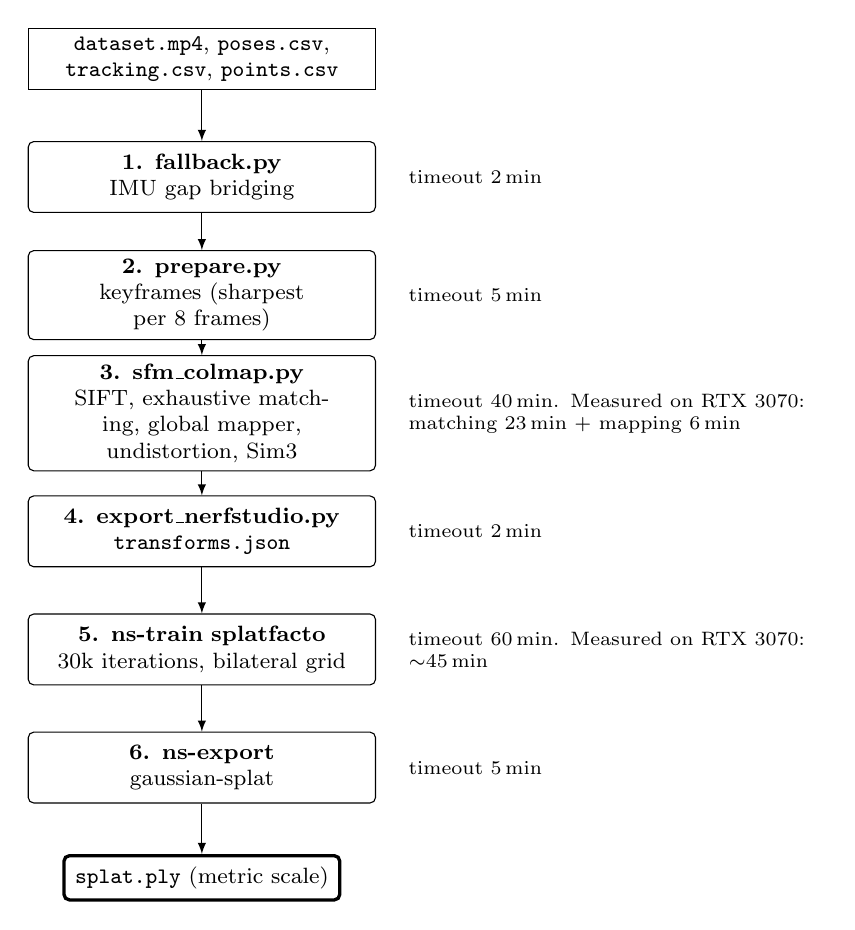
\begin{tikzpicture}[font=\footnotesize, >=latex,
  pstep/.style={draw, rectangle, rounded corners=2pt, align=center, text width=4.2cm, inner sep=3pt, minimum height=0.9cm},
  note/.style={font=\scriptsize, anchor=west, align=left, text width=5.2cm}]
  \node[draw, rectangle, align=center, text width=4.2cm, inner sep=3pt] (in) at (-2.4,1.5) {\texttt{dataset.mp4}, \texttt{poses.csv}, \texttt{tracking.csv}, \texttt{points.csv}};
  \node[pstep] (s1) at (-2.4,0)    {\textbf{1. fallback.py}\\IMU gap bridging};
  \node[pstep] (s2) at (-2.4,-1.5) {\textbf{2. prepare.py}\\keyframes (sharpest per 8 frames)};
  \node[pstep] (s3) at (-2.4,-3.0) {\textbf{3. sfm\_colmap.py}\\SIFT, exhaustive matching, global mapper, undistortion, Sim3};
  \node[pstep] (s4) at (-2.4,-4.5) {\textbf{4. export\_nerfstudio.py}\\\texttt{transforms.json}};
  \node[pstep] (s5) at (-2.4,-6.0) {\textbf{5. ns-train splatfacto}\\30k iterations, bilateral grid};
  \node[pstep] (s6) at (-2.4,-7.5) {\textbf{6. ns-export}\\gaussian-splat};
  \node[draw, very thick, rectangle, rounded corners=2pt, inner sep=4pt] (out) at (-2.4,-8.9) {\texttt{splat.ply} (metric scale)};
  \draw[->] (in) -- (s1);
  \draw[->] (s1) -- (s2);
  \draw[->] (s2) -- (s3);
  \draw[->] (s3) -- (s4);
  \draw[->] (s4) -- (s5);
  \draw[->] (s5) -- (s6);
  \draw[->] (s6) -- (out);
  \node[note] at (0.1,0)    {timeout 2\,min};
  \node[note] at (0.1,-1.5) {timeout 5\,min};
  \node[note] at (0.1,-3.0) {timeout 40\,min. Measured on RTX 3070: matching 23\,min + mapping 6\,min};
  \node[note] at (0.1,-4.5) {timeout 2\,min};
  \node[note] at (0.1,-6.0) {timeout 60\,min. Measured on RTX 3070: $\sim$45\,min};
  \node[note] at (0.1,-7.5) {timeout 5\,min};
\end{tikzpicture}
\caption{The six pipeline steps and their timeouts.}
\label{fig:pipelinesteps}
\end{figure}

\section{Android App Architecture}
Figure~\ref{fig:androidarch} shows how the capture app is put together: which class owns which output file, how the activities hand off to one another, and which files stay on the phone rather than being uploaded.


The classes are in \texttt{googleARCore/samples/hello\_ar\_java/.../helloar/}. Arrows from \texttt{HelloArActivity} show ownership or navigation by \texttt{Intent}; \texttt{CaptureLogger} feeds raw depth to \texttt{CoverageMap}. \texttt{ProcessingActivity} uploads six files plus a zipped \texttt{depth/} folder, while \texttt{camera.csv} and \texttt{anchors.csv} stay on the phone.

\begin{figure}[H]
\centering
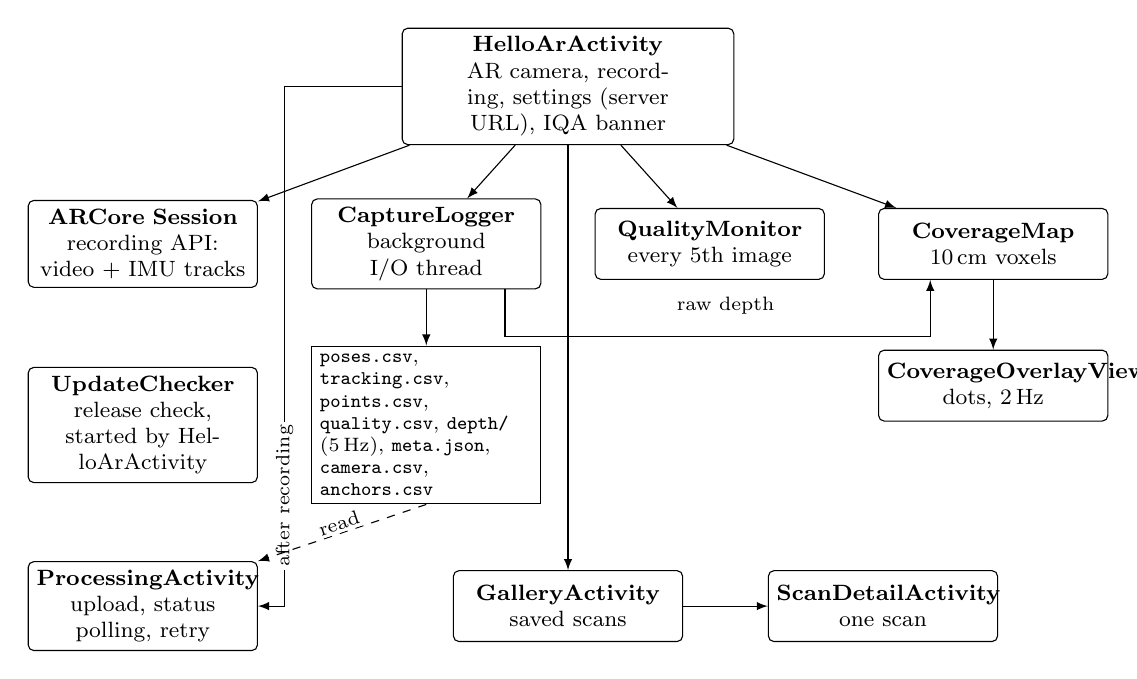
\begin{tikzpicture}[font=\footnotesize, >=latex,
  cls/.style={draw, rectangle, rounded corners=2pt, align=center, text width=2.7cm, inner sep=3pt, minimum height=0.9cm, fill=white},
  lbl/.style={font=\scriptsize, fill=white, inner sep=1pt}]
  \node[cls, text width=4.0cm] (main) at (0,3.2) {\textbf{HelloArActivity}\\AR camera, recording, settings (server URL), IQA banner};
  \node[cls] (sess) at (-5.4,1.2) {\textbf{ARCore Session}\\recording API: video + IMU tracks};
  \node[cls] (log)  at (-1.8,1.2) {\textbf{CaptureLogger}\\background I/O thread};
  \node[cls] (qm)   at (1.8,1.2)  {\textbf{QualityMonitor}\\every 5th image};
  \node[cls] (cov)  at (5.4,1.2)  {\textbf{CoverageMap}\\10\,cm voxels};
  \node[cls] (ov)   at (5.4,-0.6) {\textbf{CoverageOverlayView}\\dots, 2\,Hz};
  \node[draw, rectangle, align=left, text width=2.7cm, inner sep=3pt, font=\scriptsize] (files) at (-1.8,-1.1) {\texttt{poses.csv}, \texttt{tracking.csv}, \texttt{points.csv}, \texttt{quality.csv}, \texttt{depth/} (5\,Hz), \texttt{meta.json}, \texttt{camera.csv}, \texttt{anchors.csv}};
  \node[cls] (upd)  at (-5.4,-1.1) {\textbf{UpdateChecker}\\release check, started by HelloArActivity};
  \node[cls] (proc) at (-5.4,-3.4) {\textbf{ProcessingActivity}\\upload, status polling, retry};
  \node[cls] (gal)  at (0,-3.4)    {\textbf{GalleryActivity}\\saved scans};
  \node[cls] (det)  at (4.0,-3.4)  {\textbf{ScanDetailActivity}\\one scan};
  \draw[->] (main) -- (sess);
  \draw[->] (main) -- (log);
  \draw[->] (main) -- (qm);
  \draw[->] (main) -- (cov);
  \draw[->] (cov) -- (ov);
  \draw[->] ([xshift=1.0cm]log.south) -- ++(0,-0.6) -| ([xshift=-0.8cm]cov.south);
  \node[lbl] at (2.0,0.42) {raw depth};
  \draw[->] (log) -- (files);
  \draw[->] (main.west) -- (-3.6,3.2) -- (-3.6,-3.4) -- (proc.east);
  \node[lbl, rotate=90] at (-3.6,-2.0) {after recording};
  \draw[->] (main.south) -- (gal.north);
  \draw[->] (gal) -- (det);
  \draw[->, dashed] (files.south) -- node[lbl, sloped, above] {read} (proc.north east);
\end{tikzpicture}
\caption{Android capture app architecture.}
\label{fig:androidarch}
\end{figure}

\section{Sim3 Alignment}
Figure~\ref{fig:sim3} shows how the COLMAP reconstruction is brought into ARCore's metric frame. This is the step that gives the model its real-world scale, so every measurement in Table~\ref{tab:tape} depends on it.


The fit is done in \texttt{sfm\_colmap.py} at the export stage, with the Umeyama step unit-tested in \texttt{test\_relocalize\_and\_sfm.py}. Because ARCore re-anchors silently, only its largest self-consistent segment ends up as inliers; the inlier median residual is about 2.5\,cm. The resulting scale is validated against a tape measure (Table~\ref{tab:tape}).

\begin{figure}[H]
\centering
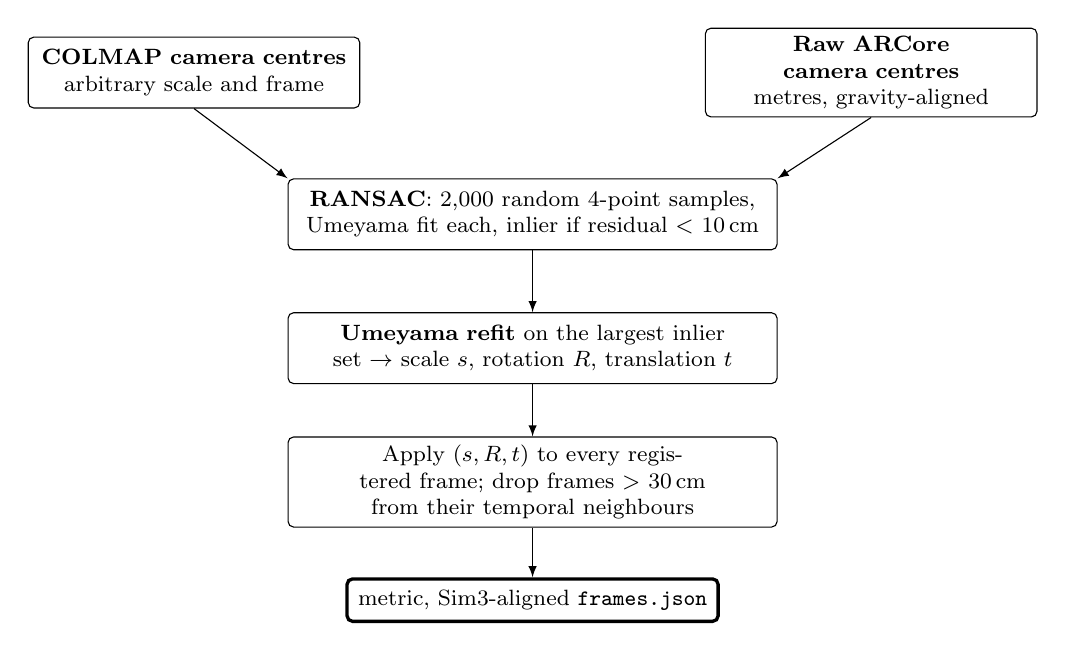
\begin{tikzpicture}[font=\footnotesize, >=latex,
  box/.style={draw, rectangle, rounded corners=2pt, align=center, text width=4.0cm, inner sep=3pt, minimum height=0.9cm}]
  \node[box] (colmap) at (-4.3,2.2) {\textbf{COLMAP camera centres}\\arbitrary scale and frame};
  \node[box] (arcore) at (4.3,2.2)  {\textbf{Raw ARCore camera centres}\\metres, gravity-aligned};
  \node[box, text width=6.0cm] (ransac) at (0,0.4) {\textbf{RANSAC}: 2{,}000 random 4-point samples, Umeyama fit each, inlier if residual $<$ 10\,cm};
  \node[box, text width=6.0cm] (refit)  at (0,-1.3) {\textbf{Umeyama refit} on the largest inlier set $\rightarrow$ scale $s$, rotation $R$, translation $t$};
  \node[box, text width=6.0cm] (apply)  at (0,-3.0) {Apply $(s, R, t)$ to every registered frame; drop frames $>$ 30\,cm from their temporal neighbours};
  \node[draw, very thick, rectangle, rounded corners=2pt, inner sep=4pt] (out) at (0,-4.5) {metric, Sim3-aligned \texttt{frames.json}};
  \draw[->] (colmap.south) -- (ransac.north west);
  \draw[->] (arcore.south) -- (ransac.north east);
  \draw[->] (ransac) -- (refit);
  \draw[->] (refit) -- (apply);
  \draw[->] (apply) -- (out);
\end{tikzpicture}
\caption{Sim3 alignment of the COLMAP reconstruction to ARCore's metric frame.}
\label{fig:sim3}
\end{figure}

\section{Coverage Map}
Figure~\ref{fig:coverage} shows how the live overlay decides a voxel's colour, which is the guidance the user acts on while walking the room.


The overlay is produced by \texttt{CoverageMap.java} and \texttt{CoverageOverlayView.java}. ARCore raw depth (5\,Hz, confidence $\geq$128, up to 5\,m) is accumulated in 10\,cm voxels, and each voxel records from which of 16 directions it was seen. Visible voxels are drawn as dots coloured by direction count, with at most 5{,}000 voxels projected and 2{,}000 dots drawn, refreshed at 2\,Hz. The grid colouring below is illustrative.

\begin{figure}[H]
\centering
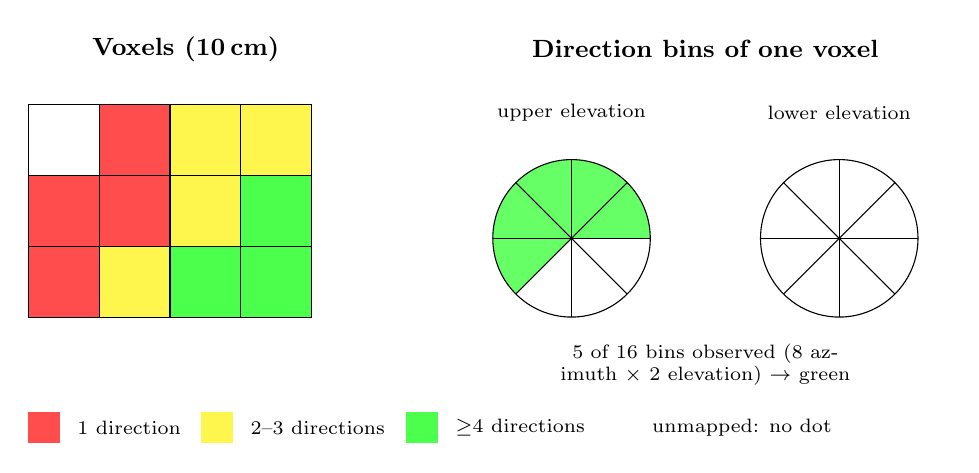
\begin{tikzpicture}[font=\footnotesize, >=latex]
  % voxel grid (illustrative colouring)
  \node[font=\small\bfseries] at (-4.0,2.4) {Voxels (10\,cm)};
  \begin{scope}[shift={(-6.0,-1.0)}]
    \foreach \x/\y/\col in {0/0/red, 1/0/yellow, 2/0/green, 3/0/green,
                            0/1/red, 1/1/red, 2/1/yellow, 3/1/green,
                            1/2/red, 2/2/yellow, 3/2/yellow} {
      \fill[\col!70] (0.9*\x,0.9*\y) rectangle ++(0.9,0.9);
    }
    \draw[step=0.9] (0,0) grid (3.6,2.7);
  \end{scope}
  % direction bins of one voxel
  \node[font=\small\bfseries, align=center] at (2.6,2.4) {Direction bins of one voxel};
  \node[font=\scriptsize] at (0.9,1.6) {upper elevation};
  \node[font=\scriptsize] at (4.3,1.6) {lower elevation};
  \foreach \a/\b in {0/45, 45/90, 90/135, 135/180, 180/225} {
    \fill[green!60] (0.9,0) -- ++(\a:1.0) arc (\a:\b:1.0) -- cycle;
  }
  \foreach \a in {0,45,90,135,180,225,270,315} {
    \draw (0.9,0) -- ++(\a:1.0);
    \draw (4.3,0) -- ++(\a:1.0);
  }
  \draw (0.9,0) circle (1.0);
  \draw (4.3,0) circle (1.0);
  \node[font=\scriptsize, align=center, text width=6cm] at (2.6,-1.6) {5 of 16 bins observed (8 azimuth $\times$ 2 elevation) $\rightarrow$ green};
  % legend
  \fill[red!70] (-6.0,-2.6) rectangle ++(0.4,0.4);
  \node[anchor=west, font=\scriptsize] at (-5.5,-2.4) {1 direction};
  \fill[yellow!70] (-3.8,-2.6) rectangle ++(0.4,0.4);
  \node[anchor=west, font=\scriptsize] at (-3.3,-2.4) {2--3 directions};
  \fill[green!70] (-1.2,-2.6) rectangle ++(0.4,0.4);
  \node[anchor=west, font=\scriptsize] at (-0.7,-2.4) {$\geq$4 directions};
  \node[anchor=west, font=\scriptsize] at (1.8,-2.4) {unmapped: no dot};
\end{tikzpicture}
\caption{Live coverage map.}
\label{fig:coverage}
\end{figure}


\section{Domain Model}
Figure~\ref{fig:domainmodel} draws the entities listed in Section~\ref{sec:domain} and the
relationships between them. The attributes shown are the fields the code actually carries, so
the diagram doubles as a map of what is written to disk at each stage.

A \textbf{Scan} produces exactly one \textbf{Dataset}; a Dataset can be submitted as more than one \textbf{Job}, because a scan may be reprocessed after a pipeline change; a Job that succeeds produces one \textbf{Model}. \textbf{Measurement} and the web-facing part of \textbf{Structural element} are FYP-2 work, drawn here because the metric scale they depend on is already established by the Sim3 step in Figure~\ref{fig:sim3}. Entity fields follow \texttt{Job} in \texttt{server/pipeline.py} and the capture files written by \texttt{CaptureLogger.java}.

\begin{figure}[H]
\centering
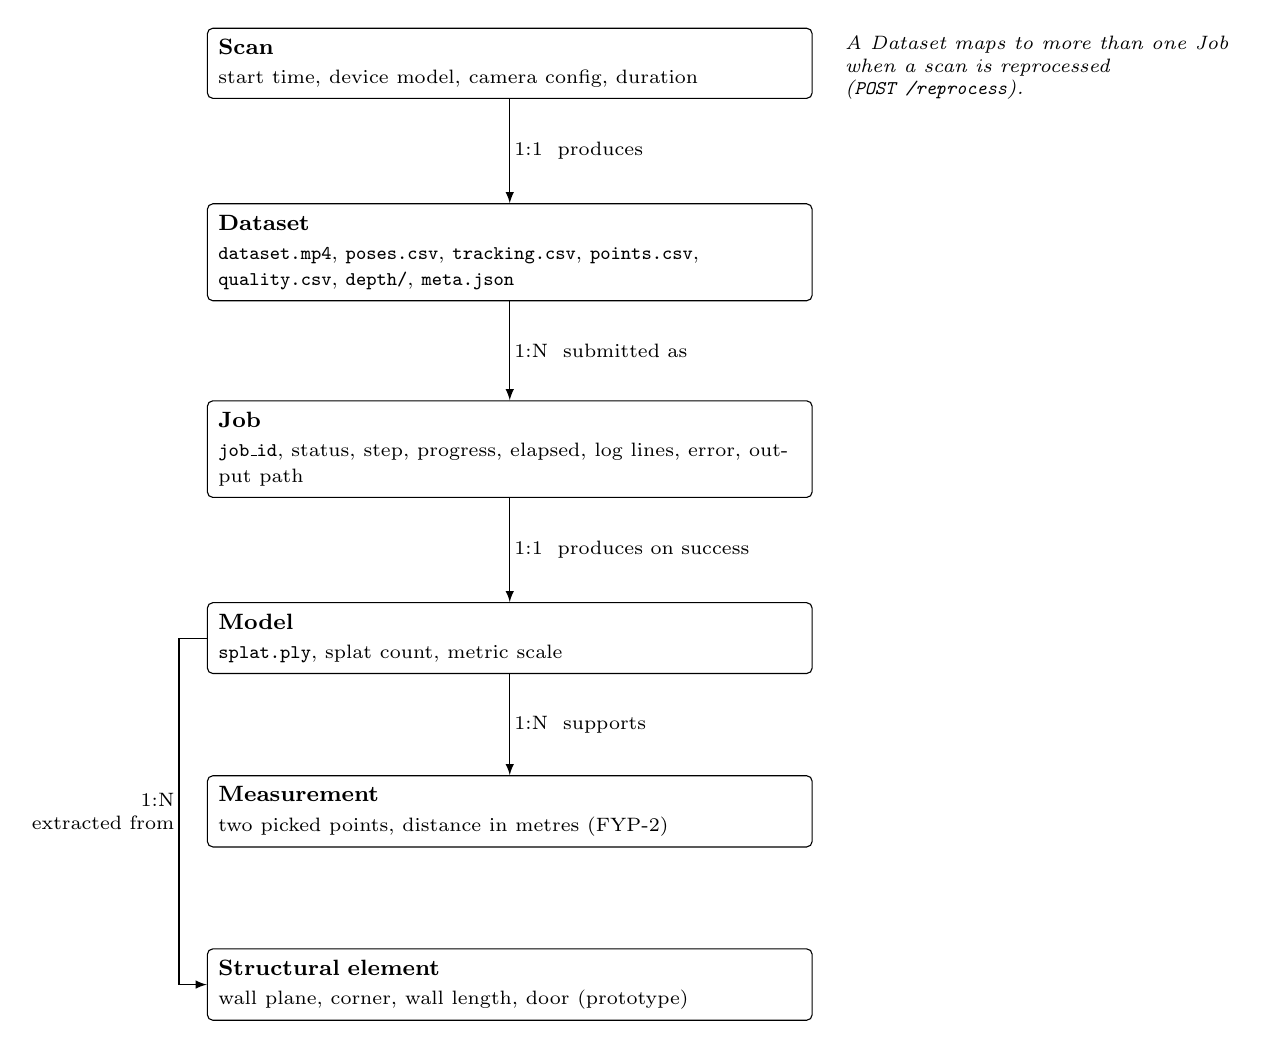
\begin{tikzpicture}[font=\footnotesize, >=latex,
  ent/.style={draw, rectangle, rounded corners=2pt, align=left, text width=7.4cm,
              inner sep=4pt, fill=white},
  rel/.style={font=\scriptsize, fill=white, inner sep=1.5pt}]

  \node[ent] (scan) at (0,5.0)
    {\textbf{Scan}\\[1pt]\scriptsize start time, device model, camera config, duration};
  \node[ent] (data) at (0,2.6)
    {\textbf{Dataset}\\[1pt]\scriptsize \texttt{dataset.mp4}, \texttt{poses.csv},
     \texttt{tracking.csv}, \texttt{points.csv}, \texttt{quality.csv},
     \texttt{depth/}, \texttt{meta.json}};
  \node[ent] (job) at (0,0.1)
    {\textbf{Job}\\[1pt]\scriptsize \texttt{job\_id}, status, step, progress, elapsed,
     log lines, error, output path};
  \node[ent] (model) at (0,-2.3)
    {\textbf{Model}\\[1pt]\scriptsize \texttt{splat.ply}, splat count, metric scale};
  \node[ent] (meas) at (0,-4.5)
    {\textbf{Measurement}\\[1pt]\scriptsize two picked points, distance in metres (FYP-2)};
  \node[ent] (struct) at (0,-6.7)
    {\textbf{Structural element}\\[1pt]\scriptsize wall plane, corner, wall length,
     door (prototype)};

  \draw[->] (scan) -- node[rel,right] {1:1 \ produces} (data);
  \draw[->] (data) -- node[rel,right] {1:N \ submitted as} (job);
  \draw[->] (job)  -- node[rel,right] {1:1 \ produces on success} (model);
  \draw[->] (model) -- node[rel,right] {1:N \ supports} (meas);
  \draw[->] (model.west) -- (-4.2,-2.3) -- (-4.2,-6.7)
        node[rel,midway,left,align=right] {1:N\\extracted from} -- (struct.west);

  \node[rel,align=left,anchor=north west] at (4.2,5.4)
    {\textit{A Dataset maps to more than one Job}\\
     \textit{when a scan is reprocessed}\\
     \textit{(\texttt{POST /reprocess}).}};
\end{tikzpicture}
\caption{Domain model entities and their relationships.}
\label{fig:domainmodel}
\end{figure}

\section{Capture Application in Use}

Figure~\ref{fig:appcapture} shows the capture app recording, with the quality and
coverage features of Figure~\ref{fig:coverage} running live on the phone.

The header confirms the capture format (1920$\times$1080 at 30\,FPS, FR-M1). The green banner is the live IQA verdict from \texttt{QualityMonitor.java}, and the row beneath it reports coverage state from \texttt{CoverageMap.java}: ceiling and floor not yet seen, and the current voxel observed from 1 of 8 azimuth directions. The red and yellow dots are the overlay drawn by \texttt{CoverageOverlayView.java}, red marking surfaces seen from a single direction and yellow from two or three. ``Searching for surfaces'' is ARCore still building its plane estimate early in the session.

\begin{figure}[H]
\centering
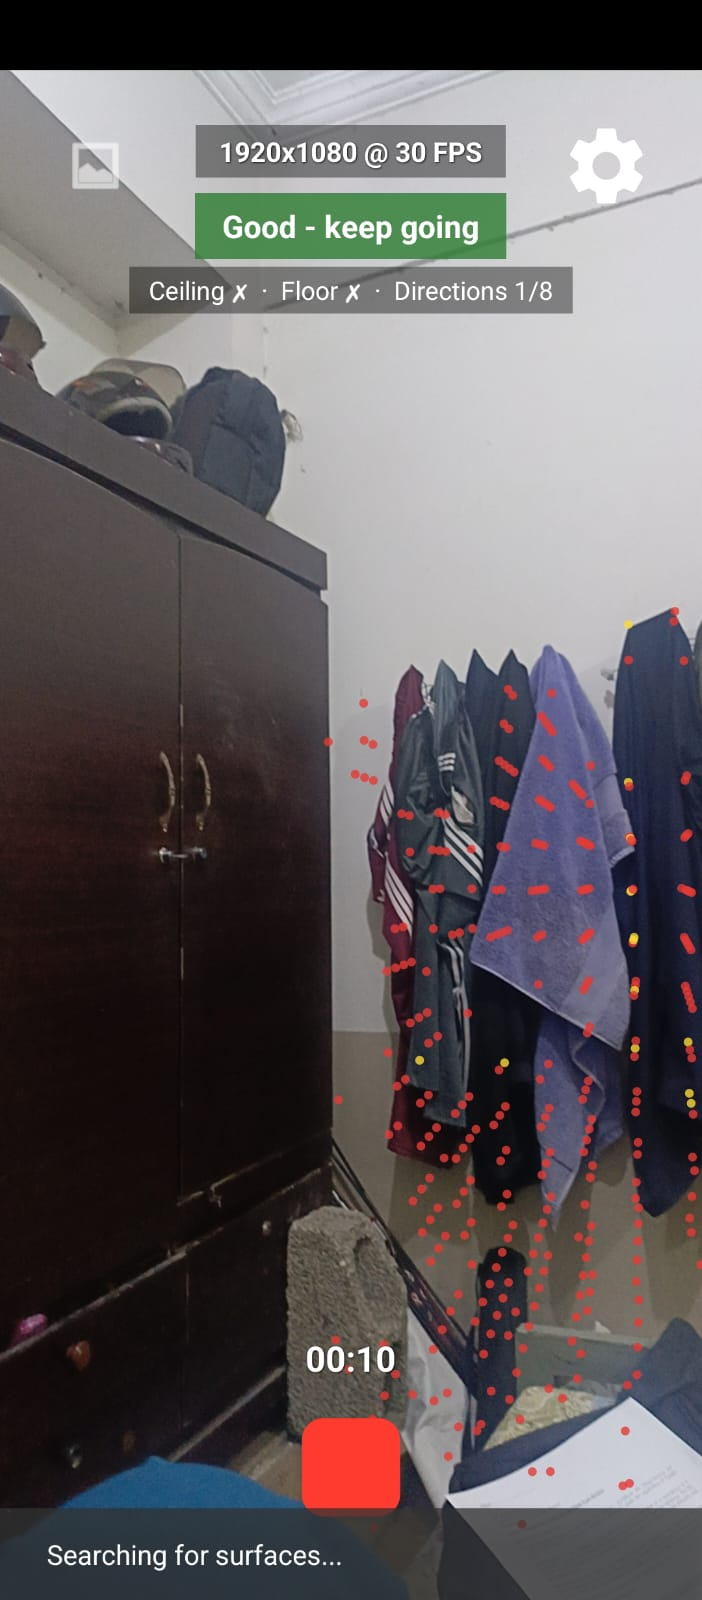
\includegraphics[height=0.62\textheight]{ThesisFigs/app-capture}
\caption{The capture app mid-recording on the realme device.}
\label{fig:appcapture}
\end{figure}
